\subsection{Selected architectural styles and patterns}

\label{sec:selected-styles-patterns}

In this section the main architectural styles and patterns are listed and described, motivating the reason why they have been chosen and how they integrate into the system architecture.

\begin{itemize}	
	\item \textbf{Client-Server architecture}: the main interaction paradigm between customers of the service and the software system is based on a \textit{request-response} model. Furthermore, interaction between Application tier and the Data tier work by means of the same paradigm. To support this kind of interaction the client-server architecture is chosen and integrated with the system trhough the introduction of servers, as shown in figure. 
	\item \textbf{Distributed Representation}: in order to keep the client side as light as possible, a client - server paradigm based on a distributed representation is chosen: all the application logic layer and the data layer are place on system side, while the presentation layer, instead, is splitted in two part:
	\begin{itemize}
		\item \textbf{System side}: the presentation layer consist in software for the generation of responses, like web pages.
		\item \textbf{Client side}: the presentation layer consist in software for the interpretation of system's responses, such as a web browser.
	\end{itemize}
	\item \textbf{4 Tiers}: the client/server architecture is split into 4 distinct tiers, decoupling data, application logic, request/response logic and client logic. As a consequence, the maintenance of the system is dramatically eased through this separation of concerns, introducing an modularity factor in the architecture.
	\item \textbf{Elastic Infrastructure}: the environment where the software system will be deployed is characterized by an unpredictable workload. To face optimaly the continuos and variable change in requests load, an elastic infrastructure is introduced to support the whole system. Through a set of API provided by the elastic infrastructure is possible to get informations about resources utilizations and to perform different tasks, even automatized, reagarding provisioning and decommissioning of IT resources.
	\item \textbf{Elastic Platform}: to get the maximum from each IT resource available, the software environment hosted by each resource, such as an operating system, can be shared among multiple components instances, for example multiple web servers or application components used by different users. As for the elastic infrastructure, the elastic platform exposes a set of API usable for provisioning and decommissioning of component instances.
	\item \textbf{Elastic Load Balancer}: to balance correctly the workload among the available resources, a load balancer is placed between the source of requests and the target. By the number of incoming requests and informations about the resources utilization, the load balancer distribute the work to the resources and can dynamically allocate more or less resources or application instances through the interface provided by the Elastic Infrastructure and the Elastic Platform.
\begin{figure}[H]
	\centerline{
		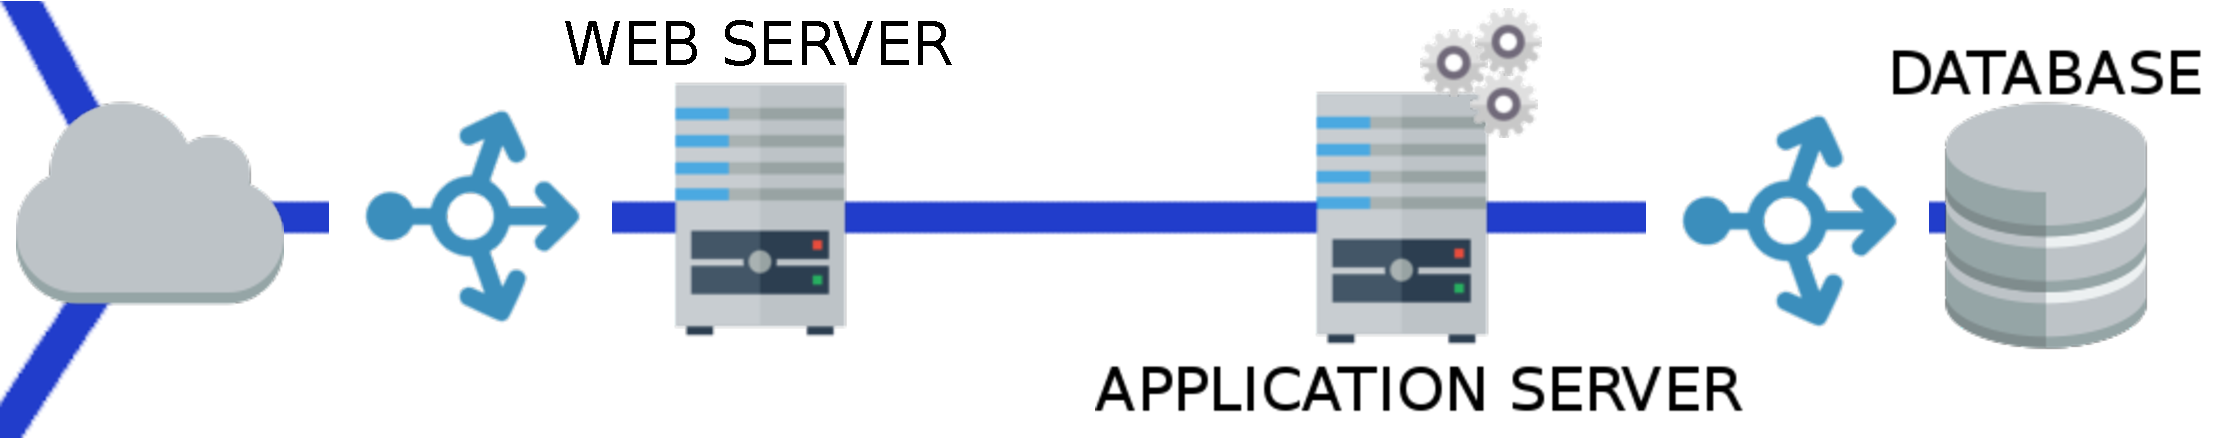
\includegraphics[width=350px]{../Datas/images/loadbalancer.pdf}
	}
	\caption{The load balancers' placement}
	\label{fig: lb-placement}
\end{figure}
\end{itemize}
